%======================================================================
%   Zak Webb
%   Ph. D. Thesis
%   Department of Physics and Astronomy
%   University of Waterloo
% 
%   Universality of single-particle scattering
%======================================================================


\documentclass[../thesis-main/thesis-main]{subfiles}
\begin{document}

\chapter{Universality of single-particle scattering}
\label{chap:SP_universality}

\todo{Edit this entire thing}

%%%%%%%%%%%%%%%%%%%%%%%%%%%%%%%%%%%%%%%%%%%%%%%%%%%%%%%%%%%%%%%%%

With the basic understanding of scattering on graphs, we should be able to combine several graphs so as to show that single-particle quantum walks are universal.  While this has already been shown by Andrew Childs \cite{Chi09}, this is a slightly different graph and analysis, which will help with the understanding of the multi-particle case.  In particular, the method for encoding a computation will be to have a long (but finite) path for each computational basis state of the circuit.  We will use several graphs from the previous section so that each gate is implemented with a scattering event.  

While the overall graph will be exponential in size, each individual scattering event will only involve either two or four semi-infinite paths, as our choice of universal gate set only mixes at most two computational basis states per gate.  As such, we will be able to analyze the evolution of a sufficiently large wavepacket, and show that the evolution of such a wavepacket follows the expected evolution for a single gate.  By then combining the graphs in such a manner, we will then be able to show that the final location of the wavepacket can be used to evaluate whether the simulated circuit accepts.


\todo{Move wavepacket propagation to this chapter?}


\section{Simulation on a quantum computer}

\todo{Show that the evolution of a nice state on an efficiently specifiable graph is contained in \BQP}


\section{Single qubit evolution}\label{sec:single_qubit_evolution}

With the understanding of single-particle graph scattering learned in \chap{scattering_on_graphs}, we will now attempt to use the various results as a computational tool.  In particular, we will now want to simulate the evolution of a quantum circuit.  To do so, we will first need to encode a single qubit.

\subsection{Single qubit encoding}\label{sec:single_qubit_encoding}

Our encoding will actually be rather simple, a dual rail encoding\todo{find where dual-rail comes from}.  A single qubit will correspond to two infinite paths, with a single wave-packet at some momentum $k$ traveling along one of the two paths.  If the particle is on the first (top) path, then the encoded qubit is in the logical state $\ket{0}$, while if the particle is on the lower graph then the encoded qubit is in the logical state $\ket{1}$.  Schematically, this can be seen in \fig{wavetrain_encoding}.

\todo{change figure to Gaussian as opposed to square?}

\begin{figure}
  \centering
  \subfloat[][]{ 
    \tikzsetnextfilename{SP_u_wavetrain0}
    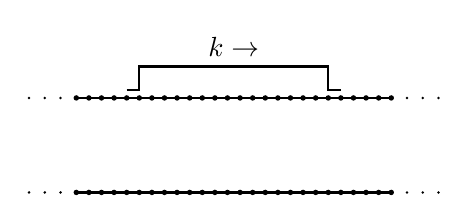
\begin{tikzpicture}[
  vert/.style={circle,fill=black,inner sep=.7pt,minimum width=0pt},
  dots/.style={circle,fill=black,inner sep=.25pt,minimum width=0pt},
  thick,
  scale=0.4]
  \foreach \x in {0,.4,...,10}{
    \node at (\x ,0) [vert]{};
    \node at (\x ,3) [vert]{};
  }

  \draw (0,0) -- (10,0);
  \draw (0,3) -- (10,3);

  \begin{scope}[yshift=0cm]
  \draw (1.6,3.25) -- (2,3.25) -- (2,4) to node [above] {$k\rightarrow$}
        (8,4) -- (8,3.25) -- (8.4,3.25);
  \end{scope}

  \foreach \xsh in {-1.5cm , 10.5cm}{
  \foreach \ysh in {0cm, 3cm}{
    \begin{scope}[xshift=\xsh,yshift=\ysh]
      \node at (0,0) [dots]{};
      \node at (0.5,0) [dots] {};
      \node at (1,0) [dots]{};
    \end{scope}
  }}
\end{tikzpicture}
    \label{fig:wavetrain0}
  }
  \qquad
  \subfloat[][]{
    \tikzsetnextfilename{SP_u_wavetrain1}
    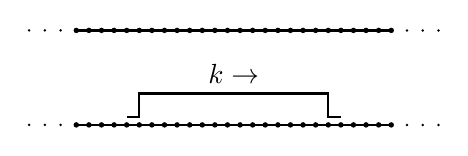
\begin{tikzpicture}[
  vert/.style={circle,fill=black,inner sep=.7pt,minimum width=0pt},
  dots/.style={circle,fill=black,inner sep=.25pt,minimum width=0pt},
  thick,
  scale=0.4]
  \foreach \x in {0,.4,...,10}{
    \node at (\x ,0) [vert]{};
    \node at (\x ,3) [vert]{};
  }

  \draw (0,0) -- (10,0);
  \draw (0,3) -- (10,3);

  \begin{scope}[yshift=-3cm]
  \draw (1.6,3.25) -- (2,3.25) -- (2,4) to node [above] {$k\rightarrow$}
        (8,4) -- (8,3.25) -- (8.4,3.25);
  \end{scope}

  \foreach \xsh in {-1.5cm , 10.5cm}{
  \foreach \ysh in {0cm, 3cm}{
    \begin{scope}[xshift=\xsh,yshift=\ysh]
      \node at (0,0) [dots]{};
      \node at (0.5,0) [dots] {};
      \node at (1,0) [dots]{};
    \end{scope}
  }}
\end{tikzpicture}
    \label{fig:wavetrain1}
   }
  \caption{A qubit is encoded using single-particle wave packets at momentum $k$.  \subfig{wavetrain0} An encoded $\ket{0}$.  \subfig{wavetrain1} An encoded $\ket{1}$.}
  \label{fig:wavetrain_encoding}
\end{figure}

Note that we implicitly assume that the wave-packet encoding the logical state of the qubit has a well-defined position, and thus that we need only measure a (relatively) small number of qubits in order to determine the location of the particle with high probability.  As such, there are actually three (or four) attributes of a Guassian wave-packet that will be of use to us: the momentum $k$, the standard deviation $\sigma$, the center of probability $\mu$, and the cutoff range $L$ (which is closely related to $\sigma$).  With these four values, and assuming that the vertices of the infinite path are labeled as $(x,j)$ for $x\in \ZZ$ and $j\in \FF_2$, we then have that the logical qubit in our system will be encoded into the states
\begin{align}
  \ket{z}_{\text{log}} = \gamma \sum_{x = \mu - L}^{\mu + L} e^{ i k x} e^{ - \frac{(x-\mu)^2}{2\sigma^2}} \ket{x,z} \label{eq:single_qubit_encoding}.
\end{align}
It is important to realize that none of these four values depend on the value of the encoded qubit; this will allow us to interfere the wave-packets arising from different paths to the same computational basis path.


This encoding is specifically chosen so that we can use \thm{single_particle_wavepacket_bound}.

\subsection{Single qubit unitary}

So far we cannot perform any interesting dynamics with our encoded qubit, as our encoding is on two (disconnected) infinite paths; there is no way for amplitude from one path to move to the second.  As such, if we want to somehow apply an encoded unitary, we will need to connect the two paths.

As \chap{scattering_on_graphs} hinted, we will do this via graph scattering.  Namely, we will examine graphs $\widehat{G}$ with four terminal vertices such that at the momentum $k$, the scattering matrices take the form
\begin{align}
  S(k) &= \begin{pmatrix} 0 & U^{T} \\
  U & 0\end{pmatrix},
  \label{eq:unitary_s_matrix}
\end{align}
where $U$ is a $2\times 2$ unitary matrix. We will use these gadgets as the connections between the two paths, so that we can perform the unitary $U$ on the encoded qubits.

More explicitly, we will have four semi-infinite paths, and we will label the four paths by $0_{\text{in}}$, $1_{\text{in}}$, $0_{\text{out}}$, and $1_{\text{out}}$ (where this labeling is the same as in equation \eq{unitary_s_matrix}).  We assume that the wave-packet encoding a qubit travels toward the graph $\widehat{G}$ along the two paths $0_{\text{in}}$ and $1_{\text{in}}$.  Far from the graph the evolution of this wavepacket is nearly identical to that of an infinite path, and thus our encoded qubit is well defined.  As the wavepacket scatters through the graph $\widehat{G}$, the state of the qubit is not particularly well defined, but after scattering, most of the amplitude is on the $0_{\text{out}}$ and $1_{\text{out}}$ paths, and is in the form of an encoded qubit.  

If we remember that $\mu$ and $k$ don't depend on the value of the initial encoded qubit, we can see that for \text{emph} encoded state, the outgoing wavepacket is well approximated by the encoded $U\ket{z}$ (where $\mu$ changes in time).  This is exactly what we were looking for.






\subsection{Single qubit unitary on a finite graph}

\todo{reorganize this entire thing}

Unfortunately, a single unitary will not be sufficient  for our purposes; while we could probably find a four-terminal graph that computes whether a given circuit accepts or rejects it's input, most of the computation would go into the construction of the graph.  As such, we will need to place multiple graphs as obstacles for the computation.  This causes problems, though, in that our construction extensively utilizes the semi-infinite paths in our analysis; we somehow need to truncate the graph.

To do this, we actually use our truncation lemma (\lem{truncation}), which does exactly this.  Assuming that two Hamiltonians are identical on some set of basis states, and assuming that the support of the initial state is far (in some specified sense) from the difference, then the evolution of the state is the same for the two Hamiltonians, up to a small error term.  By using this lemma on the scattering graph with semi-infinite paths, we can then see that if the paths are long enough (as compared to the location of the initial state), then we have a good approximation 

\lem{trunc} lets us prove analogs of \thm{singlepart} and \thm{twopart} when the graphs involved have been truncated to have finitely many vertices.

For example, consider the case where $H=H_G^{(1)}$ is the Hamiltonian \eq{single_particle_ham} for a single particle on a graph of the form shown in \fig{graph}. Let $G(K)$ be the finite graph obtained from $G$ by truncating each of the paths to have a total length $K=\Omega(L)$ (so that the endpoints of the paths are labeled $(K,j)$ for $j\in\{1,\ldots,N\}$), and choose $\tilde{H}=H_{G(K)}^{(1)}$. Let the subspace $K$ be spanned by basis states corresponding to vertices in $G(K)$.  Let $|\Phi\rangle=|\psi^j(0)\rangle$ be the same initial state as in \thm{singlepart}. We choose the evolution time $T$ so that for $0\leq t\leq T$, the time-evolved state remains far from the vertices labeled $(K,j)$ (for each $j\in\{1,\ldots,N\}$), and thus far from the effect of truncating the paths.  More precisely, we choose $T=\O(L)$ so that, for times $0\leq t\leq T$, the state $|\alpha^j (t)\rangle$ from \thm{singlepart} has no amplitude on vertices within a distance $N_0=\Omega(L)$ from the endpoints of the paths. For such times $t$ we have
\[
\left(1-P\right)H^r |\alpha^j \left(t\right)\rangle=0 \text{ for all } 0\leq  r < N_0.
\]
This allows us to use the lemma with $W=H=H_G^{(1)}$, $|\gamma(t)\rangle=|\alpha^j(t)\rangle$, and the bound $\delta=\O(L^{-{1}/{4}})$ from \thm{singlepart}. The truncation lemma then says that, for $0\leq t\leq T$,
\begin{equation}
\left\Vert \left(e^{-iH_{G}^{(1)}t}-e^{-iH_{G(K)}^{(1)}t}\right)|\psi^{j}(0)\rangle \right\Vert=\O(L^{-{1}/{4}})
\label{eq:trunc_paths}
\end{equation}
so, for $0\leq t\leq T$,
\[
\left\Vert e^{-iH_{G(K)}^{(1)}t}|\psi^{j}(0)\rangle-|\alpha^{j}(t)\rangle \right\Vert =\O(L^{-{1}/{4}}).
\]
In other words, for small enough evolution times, the conclusion of \thm{singlepart} still holds if we replace the full Hamiltonian $H^{(1)}_G$ with the truncated Hamiltonian $H_{G(K)}^{(1)}$.

In particular, let us assume that our initial states are encoded as Guassian wavepackets a distance $\mu$ from the graph, with standard deviation $\sigma$, cutoff distance $L$, and momentum $k$ (where we assume that $\mu > L$).  We will give a cutoff distance $K(k)$ and show that the evolution of our initial states on this graph are well approximated by the evolution of the same state on 

\todo{I unfortunately need to go back and prove the better bounds for the scattering state problems for the $t$ in the middle, at least for $S_{jj}(k) =0$.}

By choosing $K$ to depend on the momentum $k$, we can compensate for differing particle speeds and have the scattering process occur over a fixed amount of time, $t_{\mathrm{I}}={3L}/{2}$. As discussed in \sec{description}, we choose $K(k)=2M(k)+L$ where 
\begin{align*}
M(-{\pi}/{2}) & =  L &
M(-{\pi}/{4}) & =  \left\lceil \left(\frac{3\sqrt{2} - 2}{4}\right)L\right\rceil .
\end{align*}
 
A logical input state $a|0\rangle+b|1\rangle$ is encoded using single-particle
states $|0_{\text{\text{in}}}\rangle$ and $|1_{\text{in}}\rangle$
that only have support on the top left path and bottom left
path, respectively. The encoded states differ depending on whether
$k=-{\pi}/{2}$ or $-{\pi}/{4}$, and are defined as
\begin{align*}
|0_{\text{in}}\rangle & =  \frac{1}{\sqrt{L}}\sum_{x=M(k)+1}^{M(k)+L}e^{-ikx}|x,1\rangle &
|1_{\text{in}}\rangle & =  \frac{1}{\sqrt{L}}\sum_{x=M(k)+1}^{M(k)+L}e^{-ikx}|x,2\rangle.
\end{align*}
Starting at $t=0$ from the superposition 
\[
|\psi(0)\rangle=a|0_{\text{\text{in}}}\rangle+b|1_{\text{\text{in}}}\rangle,
\]
the computation proceeds by evolving $\ket{\psi(0)}$ with the time-independent Hamiltonian $H_{G(K)}^{(1)}$, corresponding to a quantum walk on $G(K)$. Here $K=K(k)$ but we leave the argument implicit. After time $t_{\mathrm{I}}$, the state is
\[
|\psi_{K}(t_{\mathrm{I}})\rangle=e^{-iH_{G(K)}^{(1)} t_{\mathrm{I}}}|\psi(0)\rangle.
\]
The state $|\psi_{K}(t_{\mathrm{I}})\rangle$ is approximated
by 
\begin{equation}
|\psi_{\text{out}}\rangle=\left(U_{00}a+U_{01}b\right)|0_{\text{out}}\rangle+\left(U_{10}a+U_{11}b\right)|1_{\text{out}}\rangle
\label{eq:time_evolved}
\end{equation}
where $|0_{\text{out}}\rangle$ and $|1_{\text{out}}\rangle$ are defined as
\begin{align*}
|0_{\text{out}}\rangle & =  e^{-2it_{\mathrm{I}}\cos k}\frac{1}{\sqrt{L}}\sum_{x=M(k)+1}^{M(k)+L}e^{ikx}|x,3\rangle &
|1_{\text{out}}\rangle & =  e^{-2it_{\mathrm{I}}\cos k}\frac{1}{\sqrt{L}}\sum_{x=M(k)+1}^{M(k)+L}e^{ikx}|x,4\rangle.
\end{align*}
Using the results of \sec{truncating}, the error in approximating $|\psi_{K}(t_{\mathrm{I}})\rangle$
by $|\psi_{\text{out}}\rangle$ goes to zero polynomially quickly
as $L$ grows: 
\begin{equation}
\left\Vert |\psi_{K}(t_{\mathrm{I}})\rangle-|\psi_{\text{out}}\rangle\right\Vert =\O(L^{-{1}/{4}}).
\label{eq:error_single_qubit}
\end{equation}
The effect of evolving the input state $|\psi(0)\rangle$ for time $t_{\mathrm{I}}$ is depicted in \fig{1cartoon}.



To prove equation \eq{error_single_qubit}, we write
\[
\left\Vert |\psi_{K}(t_{\mathrm{I}})\rangle-|\psi_{\text{out}}\rangle\right\Vert \leq\left\Vert |\psi_{K}(t_{\mathrm{I}})\rangle-|\psi_{\infty}(t_{\mathrm{I}})\rangle\right\Vert +\left\Vert |\psi_{\infty}(t_{\mathrm{I}})\rangle-|\psi_{\text{out}}\rangle\right\Vert .\]
We then apply the bounds
\begin{equation}
\left\Vert |\psi_{\infty}(t_{\mathrm{I}})\rangle-|\psi_{\text{out}}\rangle\right\Vert =\O(L^{-{1}/{4}})\label{eq:bound1}
\end{equation}
and
\begin{equation}
\left\Vert |\psi_{K}(t_{\mathrm{I}})\rangle-|\psi_{\infty}(t_{\mathrm{I}})\rangle\right\Vert =\O(L^{-{1}/{4}}).\label{eq:bound2}
\end{equation}
Equation \eq{bound1} follows from \thm{singlepart}.
Applying the theorem with $T=t_{\mathrm{I}}$ and $M=M(k)$, we find
\begin{equation}
\left\Vert |\psi_{\infty}(t_{\mathrm{I}})\rangle-a|\alpha^{0}(t_{\mathrm{I}})\rangle-b|\alpha^{1}(t_{\mathrm{I}})\rangle\right\Vert =\O(L^{-{1}/{4}}),\label{eq:bound_from_thm}
\end{equation}
where  
\begin{align*}
|\alpha^{0}(t_{\mathrm{I}})\rangle & =  \frac{1}{\sqrt{L}}e^{-2it_{\mathrm{I}}\cos k}\sum_{x = -\lfloor 2t_{\mathrm{I}} \sin k \rfloor-M(k)-L}^{-\lfloor 2t_{\mathrm{I}} \sin k \rfloor-M(k)-1}e^{ikx}\left(U_{00}|x,3\rangle+U_{10}|x,4\rangle\right) \\
& = \frac{1}{\sqrt{L}}e^{-2it_{\mathrm{I}}\cos k}\sum_{x=M(k)+1}^{M(k)+L}e^{ikx}\left(U_{00}|x,3\rangle+U_{10}|x,4\rangle\right) + \O(L^{-1/2})
\end{align*}
and similarly
\begin{align*}
|\alpha^{1}(t_{\mathrm{I}})\rangle & = \frac{1}{\sqrt{L}}e^{-2it_{\mathrm{I}}\cos k}\sum_{x=M(k)+1}^{M(k)+L}e^{ikx}\left(U_{01}|x,3\rangle+U_{11}|x,4\rangle\right) + \O(L^{-1/2})
\end{align*}
where the $\O(L^{-{1}/{2}})$ error terms arise from approximating the upper and lower limits of the summation. Comparing with equation \eq{time_evolved}, we see that \eq{bound_from_thm} implies \eq{bound1}.

The bound \eq{bound2} follows from equation \eq{trunc_paths} (the truncation lemma with $|\Phi\rangle  = |\psi(0)\rangle$, $H = H_{G(\infty)}^{(1)}$, $\tilde{H}  =  H_{G(K)}^{(1)}$, $W =  H$, $\delta = \O(L^{-{1}/{4}})$, $N_0 =  M(k)$, and $T = t_{\mathrm{I}}$).


\begin{figure}
  \centering
  \tikzsetnextfilename{SP_u_single_qubit_scattering_graph}
  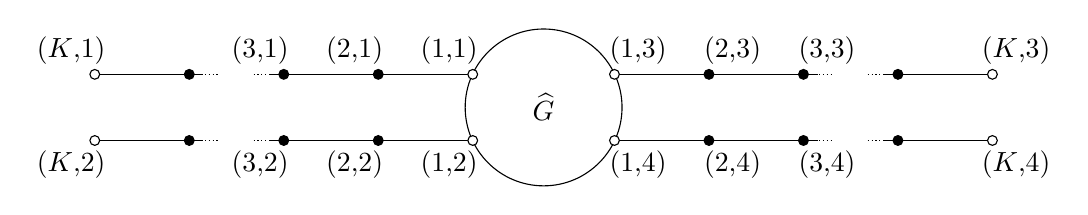
\begin{tikzpicture}[scale = 1.2,
    thin,
    attach/.style={circle,fill=white,draw=black,
      inner sep=1.25pt,minimum size=0pt},
    vert/.style={circle,draw=black,fill=black,
      inner sep=1.25pt,minimum size=0pt},
    attach/.style={circle,draw=black,fill=white,
      inner sep=1.25pt,minimum size=0pt},
    dots/.style={circle,fill=black,
      inner sep=.5pt,minimum size=0pt}]
      

   \draw (4.75,.35) circle (.83) node {$\widehat{G}$};

   \foreach \y in {0,.7}{
   \begin{scope}[yshift = \y cm]
   \draw (0,0) -- (1.15,0);
   \draw[densely dotted] (1,0) -- (1.32,0);
   \draw[densely dotted] (1.68,0) -- (2,0);
   \draw (1.85,0) -- (4,0);
   \begin{scope}[xshift=-.5cm]
   \draw (6,0) -- (8.15,0);
   \draw[densely dotted] (8,0) -- (8.32,0);
   \draw[densely dotted] (8.68,0) -- (9,0);
   \draw (8.85,0) -- (10,0);
   \end{scope}
   \foreach \x in {1,2,3,6.5,7.5,8.5}{
   \node at (\x, 0) [vert] {};}

   \node at (4,0) [attach] {};
   \node at (5.5,0) [attach]{};
   \node at (0,0) [attach] {};
   \node at (9.5,0) [attach] {};
   

   \end{scope}}
   
   
   \node[anchor=north] at (3.75,0) {(1,2)};
   \node[anchor=north] at (2.75,0) {(2,2)};
   \node[anchor=north] at (1.75,0) {(3,2)};

   \node[anchor=north] at (-.25,0) {($K$,2)};
   
   \node[anchor=south] at (3.75,.7) {(1,1)};
   \node[anchor=south] at (2.75,.7) {(2,1)};
   \node[anchor=south] at (1.75,.7) {(3,1)};

   \node[anchor=south] at (-.25,.7) {($K$,1)};
   
   \node[anchor=south] at (5.75,.7) {(1,3)};
   \node[anchor=south] at (6.75,.7) {(2,3)};
   \node[anchor=south] at (7.75,.7) {(3,3)};

   \node[anchor=south] at (9.75,.7) {($K$,3)};
      
   \node[anchor=north] at (5.75,0) {(1,4)};
   \node[anchor=north] at (6.75,0) {(2,4)};
   \node[anchor=north] at (7.75,0) {(3,4)};

   \node[anchor=north] at (9.75,0) {($K$,4)};
\end{tikzpicture}
  \label{fig:single_qubit_scattering_graph}
  \caption{A graph $G(K)$ used to perform a single-qubit gate on an encoded qubit. }
\end{figure}

\begin{figure}
  \centering
  \tikzsetnextfilename{SP_u_single_particle_cartoon}
  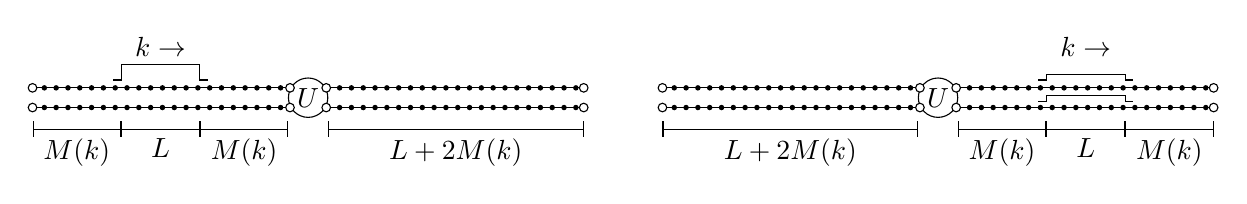
\begin{tikzpicture}[
  scale = 0.5,
  unitary/.style={circle,draw=black,fill=white,
    inner sep=0pt,minimum size=5mm},
  verts/.style={circle,fill=black,inner sep=.7pt,minimum size=0},
  attach/.style={circle,fill=white,draw=black,inner sep=1.1pt,minimum size=0pt}]
  \draw (-2,0.25) to (12,0.25);
  \draw (-2,-0.25) to (12,-0.25);

  \foreach \x in {-2,-1.7,...,12}{
  \foreach \y in {-.25,.25}{
    \node at (\x,\y) [verts] {};
  }}

  \node (1) at (5,0) [unitary] {$U$};

  \draw[xshift=-1cm] (1.05,.45) to (1.25,.45) to (1.25,.85) to (3.25,.85) 
           to (3.25,.45) to (3.45,.45);

  \node (momentum) at (1.25,1.3) [] {$k\rightarrow$};

  \draw[|-|] (-2,-.8)   to node[below] {$M(k)$} (0.25,-.8);
  \draw[|-|] (0.25,-.8) to node[below] {$L$}   (2.25,-.8);
  \draw[|-|] (2.25,-.8) to node[below] {$M(k)$} (4.5,-.8); 

  \draw[|-|] (5.5,-.8) to node[below] {$L + 2M(k)$} (12,-.8);

  \foreach \x in {-2, 12, 4.54, 5.46}{
  \foreach \y in {-.25, .25}{  
    \node at (\x,\y) [attach]{};
  }}

\begin{scope}[xshift=4cm]
  \draw (10,0.25) to (24,0.25);
  \draw (10,-0.25) to (24,-0.25);
  
  \foreach \x in {10,10.3,...,24}{
  \foreach \y in {-.25,.25}{
    \node at (\x,\y) [verts] {};
  }}
  
  \node (2) at (17,0) [unitary] {$U$};
 
  \draw[xshift=1cm] (18.55,.45) to (18.75,.45) to (18.75,.6)
     to (20.75,.6) to (20.75,.45) to (20.95,.45);

  \draw[xshift=1cm] (18.55,-.1) to (18.75,-.1) to (18.75,.05)
     to (20.75,.05) to (20.75,-.1) to (20.95,-.1);

  \node (momentum2) at (20.75,1.3) [] {$k\rightarrow$};


  \draw[|-|] (10,-.8) to node[below] {$L+2M(k)$} (16.5,-.8);
  \draw[|-|] (17.5,-.8) to node[below] {$M(k)$} (19.75,-.8);
  \draw[|-|] (19.75,-.8) to node[below] {$L$} (21.75,-.8);
  \draw[|-|] (21.75,-.8) to node[below] {$M(k)$} (24,-.8);
  
  \foreach \x in {10, 24, 16.54, 17.46}{
  \foreach \y in {-.25, .25}{  
    \node at (\x,\y) [attach]{};
  }}
\end{scope}
\end{tikzpicture}
  \caption{A single-qubit gate $U$ acts on an encoded qubit. The wave packet starts on the paths on the left-hand side of the figure, a distance $M(k)$ from the ends of the paths. After time $t_{\mathrm{I}}={3L}/{2}$ the logical gate has been applied and the wave packet has traveled a distance $2M(k)+L$ (up to error terms that are bounded as $\O(L^{-{1}/{4}}))$.}
  \label{fig:single_particle_cartoon}
\end{figure}

\subsection{Multi-gate computations}

\todo{talk about combining graphs, and then use the truncation lemma}.

\todo{make a figure}

\subsection{Explicit encodings}

\todo{Find universal gate set for several momenta ($\pi/2$, $\pi/4$, $\pi/3$, etc.)}



%%%%%%%%%%%%%%%%%%%%%%%%%%%%%%%%%%%%%%%%%%%%%%%%%%%%%%%%%%%%%%%%%

\section{Multi-qubit computations}
\label{sec:multi_qubit_computations}

Now that we have a decent understanding of a single qubit computation, we now need to understand multi-qubit computations.  The intuitive construction will remain the same, but the requisite number of vertices will become rather large.  In particular, our construction will require an exponential number of long paths.  This exponential size is required, however, as the Hilbert space of a single-particle quantum walk is only as large as the number of vertices of the graph

\subsection{Encoding qubits}\label{sec:multi_qubit_encoding}

Let us now give the encoding of $n$ qubits in our scattering framework.  As in \sec{single_qubit_encoding}, we will encode the state as a wave-packet traveling along an infinite path, where the value of the qubit is encoded in the path on which the particle is located.  For a single qubit, this meant that we had two infinite paths, corresponding to logical $0$ and $1$.  For $n$ qubits, however, this means that we need $2^n$ infinite paths, one path corresponding to each basis state.

We will still have four important quantities that are independent of the state of the qubit, namely the momentum of the wave-packet $k$, the position of the center of the wave-packet $\mu$ (which does depend on $t$), the cutoff distance $L$, and the standard deviation of the Guassian $\sigma$.  As such, if we label the $2^n$ infinite paths by the strings $\mathbf{z}\in \FF_2^n$, and the vertices as $(x,\mathbf{s})$ for $x\in \ZZ$ and $\mathbf{z}\in \FF_2^n$, we have that the logical states are encoded in the wave-packets
\begin{align}
  \ket{\mathbf{z}}_{\text{log}} = \gamma \sum_{x = \mu - L}^{\mu + L} e^{ i k x} e^{ - \frac{(x-\mu)^2}{2\sigma^2}} \ket{x,\mathbf{z}} \label{eq:multi_qubit_encoding}.
\end{align}
Note that we again use this construction so that we will be able to analyze the dynamics via \thm{single_particle_wavepacket_bound}.


\subsection{Single gates}

We will perform 
  
\subsection{Stupid stuff to fix}

Before we encode an entire computation into the evolution of a quantum walker, we first need to be able to encode a single gate.  To do this, we will use the results of \chap{scattering_on_graphs}, as we have already shown how to simulate the evolution of a universal gate set.  Unfortunately, the results of that section do require that each of the input and output paths to be semi-infinite, which will be problematic for combining these evolutions in series.

However, if we examine \lem{SP_wavepacket}, we can see that for all times of interest, most of the amplitude remains close to the graph.  Intuitively, we would thus expect the evolution for these times to remain mostly unchanged if we then remove those vertices far from the graph.  This is actually the bulk of the \lem{NPL}, which we will use to great effect in our proof.

Before we analyze the actual evolution, however, we will want to construct these small graphs themselves.  As such, let us assume that we are working with $n$ qubits, and let us assume that we are applying the unitary $U$, where $U\in \{H, T,\CNOT\}$.  With this assumption, the graph corresponding to  a single gate will then consist of $2^{n+1}$ paths of length $2M+L$, where $M$ and $L$ are integers to be determined, along with a scattering graph $G_U$ that implements the appropriate unitary evolution.  Half of the long paths will correspond to the input paths, while the other half will correspond to the output paths.  We will then connect these paths to the input and output vertices of $G_U$.   In particular, the graph will look like \fig{SP_block}.  

\todo{fix figure, for single qubit case}

\begin{figure}
  \centering
  \tikzsetnextfilename{SP_block}
  %%%%%%%%%%%%%%%%%%%
%  This is the TikZ code for the single-particle block idea.  In particular, this contains code for stuff.
%

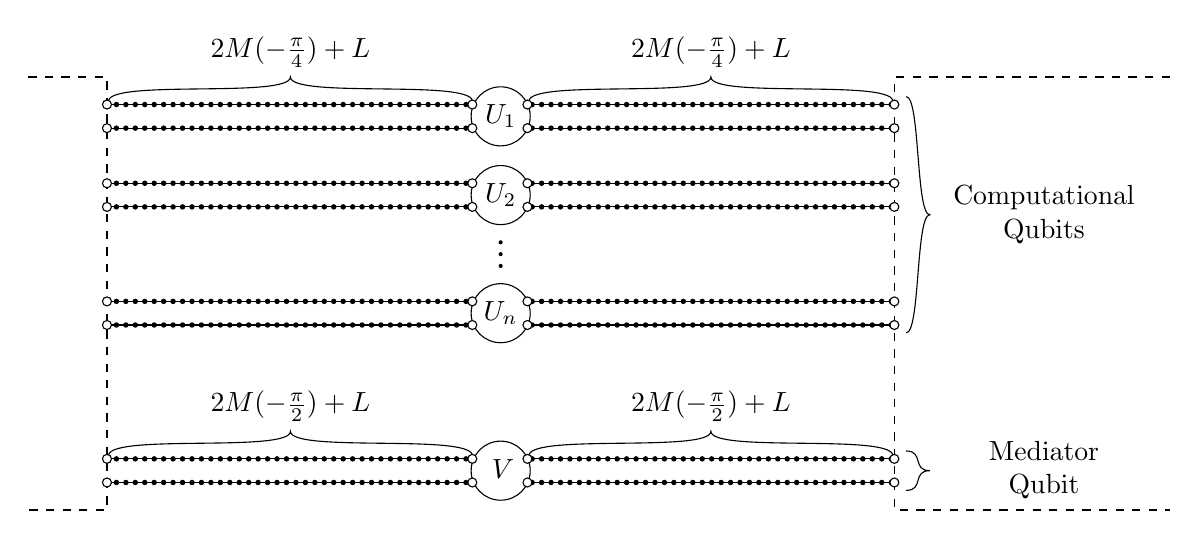
\begin{tikzpicture}[
  unitary/.style={circle,draw=black,fill=white,
    inner sep=0pt,minimum size=7.5mm},
  dots/.style={circle,fill=black,
    inner sep=0pt,minimum size=1.5pt},
  vert/.style={circle,fill=black,
    inner sep=.7pt,minimum size=0pt},
  attach/.style={circle,draw=black,fill=white,inner sep=1.15pt,minimum size=0}]

  \foreach \n /\y in {U_1/2.5,U_2/1.5,U_n/0,{V_{\med}}/-2}{
    \begin{scope}[yshift = \y cm]
      \foreach \x in {0,.12,...,10} {
        \node at (\x, -.15) [vert] {};
        \node at (\x, .15) [vert] {};
      }
      \draw (0, -.15) to (10, -.15);
      \draw (0,  .15) to (10,  .15);
      \node at (5,0) [unitary]{$ \n $};


    \end{scope}
  }
  
  \foreach \x in {0,5.34}{
  \foreach \y /\p in {2.5/4,-2/2}{
  \begin{scope}[xshift=\x cm,yshift=\y cm]
    \node (\x\p) at (2.33,.5)[above] {$2M(-\frac{\pi}{\p}) + L$};
  
    \draw (0.02,0.2) to[out=80,in=-90,looseness=0.3] (2.33,.5)
                     to[out=-90,in=100,looseness=0.3] (4.64,.2);
  \end{scope}}} 
                  
  \draw (10.15,2.75) to[out=0,in=-180,looseness=0.3] (10.45,1.25)
                    to[out=-180,in=0,looseness=0.3] (10.15,-.25);
  \node at (11.9,1.25)
      {\begin{tabular}{c}
          Computational\\ 
          Qubits\end{tabular}};


  \draw (-1,3) to (0, 3) to (0,-2.5) to (-1,-2.5) [dashed];
  \draw (13.5,3) to (10,3) to (10,-2.5) to (13.5,-2.5) [dashed];

  \node at (5,.9) [dots] {};
  \node at (5,.75)    [dots] {};
  \node at (5,.6) [dots] {};

  \draw (10.15,-1.75) to[out=0,in=-180,looseness=1.5] (10.45,-2)
                    to[out=-180,in=0,looseness=1.5] (10.15,-2.25);
  \node at (11.9,-2) 
      {\begin{tabular}{c}
          Mediator\\ 
          Qubit\end{tabular}};
          
   \foreach \x in {0, 10, 4.64, 5.34}{
   \foreach \y in {2.35,2.65,1.65,1.35,.15,-.15,-1.85,-2.15}{
     \node at (\x, \y) [attach] {};
   }}
\end{tikzpicture}
  \caption{The intuitive idea for a single-particle block.}
  \label{fig:SP_block}
\end{figure}

Additionally, as the scattering behavior of graphs is intrinsically related to the momentum of the wavepackets, we will need to decide on this before we finish the construction.  In anticipation of \chap{MP_universality}, as well as the simplicity of certain graphs, our construction will utilize $k = -\dfrac{\pi}{4}$.

%%%%%%%%%%%%%%%%
\subsection{Construction of $G_U$}

With these choices, the graphs for $G_U$ will be relatively simple.  For all graphs except for the amplitude mixing gate, the subgraphs will simply consist of paths, so that the evolution will essentially just be the same as on a long path, possibly with an encoded change of phase.  For the amplitude mixing gate, things will be slightly di

If $U$ is a $\Tgate$-gate acting on qubit $j$, then the graph $G_U$ will consist of $2^{n-1}$ paths of length $2$ connecting input $x_{\text{in}}$ to $x_{\text{out}}$, where $x_j = 0$, and $2^{n-1}$ paths of length $1$ connecting input $x_{\text{in}}$ to output $x_{\text{out}}$ where $x_{j} = 1$.  In this manner, the scattering amplitude will always have perfect transmision, and different momenta will only result in a different encoded gate (namely that this will be a $-\dfrac{k}{2}$-phase gate as opposed to a $\dfrac{\pi}{8}$-gate.

If $U$ is a $\CNOT$-gate controlled by qubit $i$ and acting on qubit $j$, then this is even more simple than the $\Tgate$-gate.  In particular, the graph $G_U$ will consist of $2^n$ paths of length 2, where input $x$ is connected to output $y$, where $x_k = y_k$ for all $k\neq j$, and $y_j =x_i + x_j - 2 x_i x_j$. 

Finally, if $U$ is the Basis-changing gate acting on qubit $j$, then things become slightly more complicated.  In particular, $G_U$ then consists of $2^{n-1}$ copies of the graph \fig{basis_change}, with inputs $x_{\text{input}}$ and $y_{\text{input}}$ with $x_i = y_i$ for all $i\neq j$, and $x_j = 1-y_j$, and outputs $x_{\text{out}}$ and $y_{\text{out}}$.

These are represented pictorially in \fig{SP_G_U}.  Note that the paths corresponding to the basis states are ordered to make the figures coherent, and that the ordering depends on which qubits the gate acts.

\todo{make figure}


%%%%%%%%%%%%%%%%
\subsection{Evolution analysis}

An important aspect to note about this graph is that while $G_U$ has exponentially many inputs and outputs, it actually consists of either $2^n$ or $2^{n-1}$ disconnected graphs, as our universal gate set only ever mixes at most two basis states.  As such, each scattering event will only ever deal with finite sized graphs, and we will be able to use \lem{SP_wavepacket} without worry.

In particular, if we assume that the initial state is a superposition of square wavepackets that are all a distance $M$ from the 


%%%%%%%%%%%%%%%%%%%%%%%%%%%%%%%%%%%%%%%%%%%%%%%%%%%%%%%%%%%%%%%%%

\section{Combining blocks}

With the understanding of exactly how a single graphs block is expected to simulate a single circuit, we will want to understand how to combine these blocks so as to be able to perform a simulation of an entire circuit.  

%%%%%%%%%%%%%%%%%%%%%%%%%%%%%%%%%%%%%%%%%%%%%%%%%%%%%%%%%%%%%%%%%




%%%%%%%%%%%%%%%%%%%%%%%%%%%%%%%%%%%%%%%%%%%%%%%%%%%%%%%%%%%%%%%%%

\section{Discussion and extensions}

What else can go here?

%%%%%%%%%%%%%%%%%%%%%%%%%%%%%%%%%%%%%%%%%%%%%%%%%%%%%%%%%%%%%%%%%

\biblio

\end{document}